
\begin{tikzpicture}[line width=1.1mm]
\node[draw,scale=2,fill=blue!20!red]{Extras};
\end{tikzpicture}

%\begin{tikzpicture}\draw[help lines] %(0,0)grid(3,2);\coordinate(a)at %(1,0);\coordinate(b)at (3,1);\draw(a)-- %(b);\coordinate(c)at ($ (a)!.25!(b) %$);\coordinate(d)at ($ %(c)!1cm!90:(b)$);\draw[<->] (c)-- %(d)node[sloped,midway,above] {  1cm}
%\end{tikzpicture}


\tdplotsetmaincoords{60}{120}
\begin{tikzpicture}[tdplot_main_coords]

  % axes
  \draw[thick,->] (0,0,0) -- ( 5,0,0) node[anchor=south]{$x$};
  \draw[thick,->] (0,0,0) -- ( 0,4,0) node[anchor=west]{$y$};
  \draw[thick,->] (0,0,0) -- ( 0,0,5) node[anchor=north east]{$-z$};  
  \draw[thick]    (0,0,0) -- ( 0,-2,0);
  \draw[thick,->] (0,0,0) -- ( 0,0,-3) node[anchor=south west]{$z$};

  % vector 1
  \pgfmathsetmacro{\ax}{5}
  \pgfmathsetmacro{\ay}{5}
  \pgfmathsetmacro{\az}{2}
  \draw[very thick,->,red] (0,0,0) -- (\ax,\ay,\az) node[anchor=west]{source};

   % vector 2
  \pgfmathsetmacro{\bx}{-2}
  \pgfmathsetmacro{\by}{-2}
  \pgfmathsetmacro{\bz}{2}
  \draw[very thick,->,blue] (0,0,0) -- (\bx,\by,\bz) node[anchor=north]{sim};

   % vector 3 (projection)
  \pgfmathsetmacro{\cx}{\ax*1.2}
  \pgfmathsetmacro{\cy}{0}
  \pgfmathsetmacro{\cz}{\az*1.2}
  \draw[very thick,green] (0,0,0) -- (\cx,\cy,\cz);

   % dashed lines
%  \draw[dashed,gray] (\ax,\ay,\az) -- (\ax,\ay,0);
  \draw[dashed,gray] (\ax,\ay,\az) -- (\ax,0,\az);
  \draw[dashed,gray] (\ax,\ay,\az) -- (0,\ay,\az);
%  \draw[dashed,gray] (\ax,0,0) -- (\ax,\ay,0) -- (0,\ay,0);
  \draw[dashed,gray] (\ax,0,0) -- (\ax,0,\az) -- (0,0,\az);
  \draw[dashed,gray] (0,0,\az) -- (0,\ay,\az) -- (0,\ay,0);

  % arcs
  \tdplotdefinepoints(0,0,0)(\ax,\ay,\az)(\bx,\by,\bz)
  \tdplotdrawpolytopearc[<->]{2}{anchor=north west}{$\theta$}
  \tdplotdefinepoints(0,0,0)(0,0,1)(\bx,\by,\bz)
  \tdplotdrawpolytopearc[<->]{3}{anchor=north}{$\beta$}
  \tdplotdefinepoints(0,0,0)(1,0,0)(\cx,\cy,\cz)
  \tdplotdrawpolytopearc[<->]{1}{anchor=north}{$\phi$}

\end{tikzpicture}

\vspace{1cm}

%\setlength{\unitlength}{0.20mm} %zoom
%\begin{picture}(400,250) %tamanho
%\put(75,10){\line(1,0){130}}
%\put(75,50){\line(1,0){130}}
%\put(75,200){\line(1,0){130}}
%\put(120,200){\thicklines{\vector(0,-1){150}}}
%\put(190,200){\thicklines{\vector(0,-1){190}}}
%\put(97,120){$\alpha$}
%\put(170,120){$\beta$}
%\put(220,195){upper state}
%\put(220,45){lower state 1}
%\put(220,5){lower state 2}
%\end{picture}


\begin{tikzpicture}[line width=1.1mm]
\node[draw,scale=2,fill=blue!20!red]{Plano inclinado};
\end{tikzpicture}

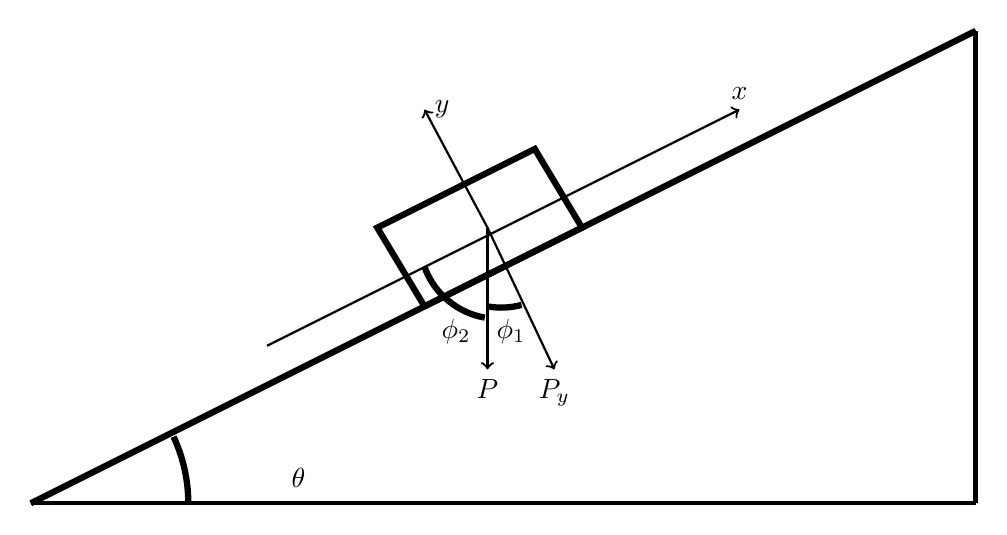
\begin{tikzpicture}[line width=0.8mm]
% Plano inclinado
  \coordinate (v1) at (-6,0);
  \coordinate (v2) at (6,0);
  \coordinate (v3) at (6,6);
  \draw  (v3) -- (v1);
  \draw[ultra thick,-] (v1) --(v2);
  \draw[ultra thick,-] (v1) -- (v3);
  \draw[ultra thick,-] (v2) -- (v3);
  % add coordinate at the extension of the line from v1 to v2.
  %o primeiro termo entre colchetes acima, seleciona o tamanho da fonte
  %já o último termo posiciona a figura.
  
  %quadrado
  \coordinate (v4) at (-1,2.5);
  \coordinate (v5) at (-1.6,3.5);
  \coordinate (v6) at (0.4,4.5);
  \coordinate (v7) at (1,3.5);
  \draw (v4) -- (v5) -- (v6) -- (v7) -- (v4);
  
  % Eixos
  \draw[thick,->] (-3,2) -- ( 3,5) node[anchor=south]{$x$};
  \draw[thick,->] (-0.2,3.5) -- ( -1,5) node[anchor=west]{$y$};
  \draw[thick,->] (-0.2,3.5) -- ( 0.65,1.7) node[anchor=north]{$\Vec{P_{y}}$};
  \draw[thick,->] (-0.2,3.5) -- (-0.2,1.7) node[anchor=north]{$\Vec{P}$};
  
  % arcs
  \draw (-4,0) arc (0:25:2);
  \node[anchor=north] at (-2.6,0.6) {$\theta$};
  \draw (-1,3) arc (200:260:1);
  \node[anchor=north] at (-0.6,2.5) {$\phi_{2}$};
  \draw (-0.2,2.5) arc (260:285:1);
  \node[anchor=north] at (0.1,2.5) {$\phi_{1}$};

\end{tikzpicture}

\tdplotsetmaincoords{60}{120}
\begin{tikzpicture}[tdplot_main_coords]

  % axes
  \draw[dashed,thick,->] (-7,0,0) -- ( 7,0,0) node[anchor=west]{$x$};
  \draw[dashed,thick,->] (0,-3,0) -- ( 0,4,0) node[anchor=west]{$y$};
  \draw[dashed,thick,->] (0,0,0) -- ( 0,0,5) node[anchor=west]{$z$};

  % vetor 1
  \pgfmathsetmacro{\ax}{6}
  \pgfmathsetmacro{\ay}{-3}
  \pgfmathsetmacro{\az}{0}
  \draw[very thick,<-,red] (0,0,0) --node[anchor=south ]{\fontsize{14pt}{14pt}\selectfont$\vec{r}_{BO}$} (\ax,\ay,\az);
  % vetor 2
  \draw[very thick,brown] (0,0,\az) --node[left]{\fontsize{14pt}{14pt}\selectfont$3m$} (0,0,4);
  % vetor 3
  \draw[very thick,blue] (\ax,0,0) --node[anchor=north]{\fontsize{14pt}{14pt}\selectfont$1,25m$} (\ax,\ay,\az);
  \draw[very thick,blue] (\ax,0,\az) --node[right]{\fontsize{14pt}{14pt}\selectfont$2m$} (0,0,\az);
  % vetor 4
  \draw[very thick,<-,orange] (0,0,4) --node[left ]{\fontsize{15pt}{15pt}\selectfont$\vec{F}_{AB}$} (\ax,\ay,\az);
  % vetor 5
  \draw[very thick,->,brown] (0,0,\az) --node[right]{\fontsize{16pt}{16pt}\selectfont$\vec{P}$} (0,0,-4);
  % vetor 6
  \draw[very thick,->,purple] (-3,0,\az) --node[right ]{\fontsize{15pt}{15pt}\selectfont$\vec{F}_{AC}$} (0,0,4);
  \draw[very thick,black] (-3,0,\az) --node[right]{\fontsize{14pt}{14pt}\selectfont$1m$} (0,0,\az);
  
  % arcs
  \tdplotdefinepoints(\ax,\ay,\az)(0,0,0)(0,0,4)
  \tdplotdrawpolytopearc[-]{2}{right}{$\theta$}
  \tdplotdefinepoints(-\ax,-\ay,0)(0,0,0)(-\ax,0,0)
  \tdplotdrawpolytopearc[-]{1.5}{right}{$\psi$}
  \tdplotdefinepoints(-3,0,0)(0,0,0)(0,0,4)
  \tdplotdrawpolytopearc[-]{1.5}{left}{$\phi$}

   % dashed plano
  \draw[dashed,gray] (-\ax,\ay,0) -- (\ax,\ay,0);
  \draw[dashed,gray] (\ax,-\ay,0) -- (\ax,\ay,0);
  \draw[dashed,gray] (-\ax,-\ay,0) -- (-\ax,\ay,0);
  \draw[dashed,gray] (\ax,-\ay,0) -- (-\ax,-\ay,0);
  
\end{tikzpicture}


\begin{tikzpicture}[line width=1.1mm]
\node[draw,scale=2,fill=blue!20!red]{Lei dos Senos};
\end{tikzpicture}

\begin{tikzpicture}[line width=0.7mm]
  \coordinate (v1) at (-6,0);
  \coordinate (v2) at (-1,6);
  \coordinate (v3) at (6,0);
  % add coordinate at the extension of the line from v1 to v2
  \coordinate (v2) at ($(v1)!1.2!(v2)$); 
  \draw (v1) -- node[font=\fontsize{16pt}{16pt}\selectfont,left,xshift=-0.5cm] {$F_{2}$} (v2) ;
  \draw (v2) -- node[font=\fontsize{16pt}{16pt}\selectfont,right,xshift=0.2cm] {$F_{1}$}(v3);
  \draw  (v3) -- node[font=\fontsize{16pt}{16pt}\selectfont,anchor=north] {$F_{3}$}(v1);
  
  % arcs
  \draw (-5,0) arc (0:28:2);
  \node[font=\fontsize{16pt}{16pt}\selectfont,anchor=north west] at (-4.8,0.9) {$\theta_{23}$};
  \draw (-0.5,6.55) arc (200:330:0.6);
  \node[font=\fontsize{16pt}{16pt}\selectfont,left] at (0,5.9) {$b$};
  \node[font=\fontsize{16pt}{16pt}\selectfont,right] at (0,5.9) {$a$};
  \draw (5,0) arc (180:130:1);
  \node[font=\fontsize{16pt}{16pt}\selectfont,anchor=north east] at (4.8,0.9) {$\theta_{13}$};
  
  % axes
  \draw[dashed,thick,->] (0,0) -- node[font=\fontsize{16pt}{16pt}\selectfont,left]{$h$}(v2) ;
\end{tikzpicture}

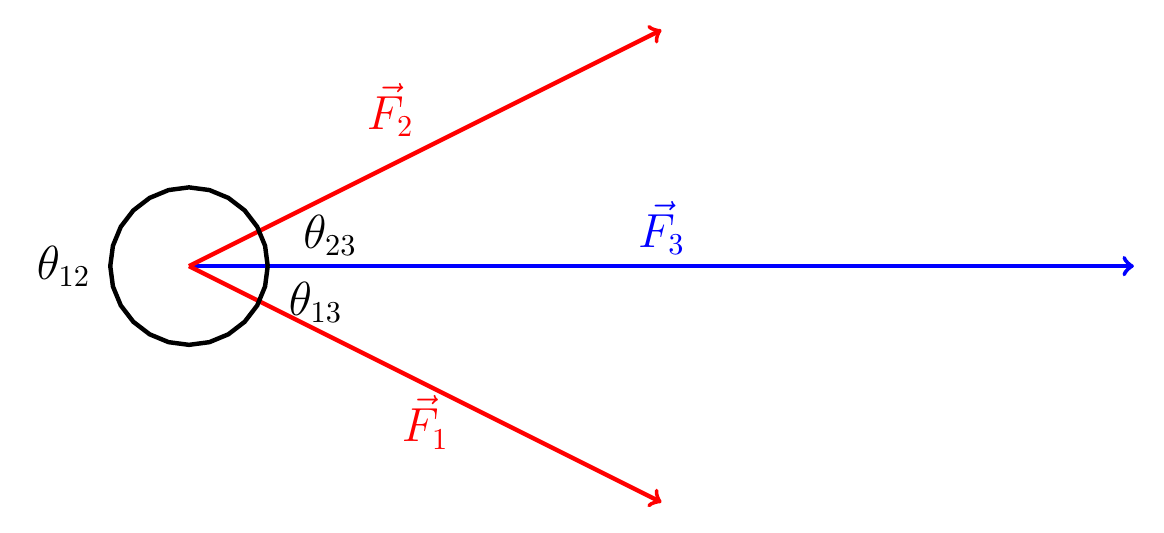
\begin{tikzpicture}[line width=0.7mm]
  \coordinate (v1) at (12,0);
  \coordinate (v3) at (0,0);
  \coordinate (v4) at (6,3);
  \coordinate (v5) at (6,-3);
  % add coordinate at the extension of the line from v1 to v2
 
  %o primeiro termo entre colchetes acima, seleciona o tamanho da fonte
  %já o último termo posiciona a figura
  \draw[blue,ultra thick,<-]  (v1) -- node[font=\fontsize{16pt}{16pt}\selectfont,above] {$\vec{F_{3}}$}(v3);
  %rótulo das alturas,lados...
  \draw[red,ultra thick,->] (v3) --node[font=\fontsize{16pt}{16pt}\selectfont,below] {$\vec{F}_{1}$} (v5);
  \draw[red,ultra thick,->] (v3) --node[font=\fontsize{16pt}{16pt}\selectfont,above left] {$\vec{F}_{2}$} (v4);
  
  % arcs
  \draw [ultra thick,domain=0:360] plot({cos(\x)},{sin(\x)});
  \node[font=\fontsize{16pt}{16pt}\selectfont,anchor=north west] at (1.3,0.8) {$\theta_{23}$};
  \node[font=\fontsize{16pt}{16pt}\selectfont,left] at (-1.1,0) {$\theta_{12}$};
  \node[font=\fontsize{16pt}{16pt}\selectfont,anchor=north east] at (2.1,-0.05) {$\theta_{13}$};
\end{tikzpicture}

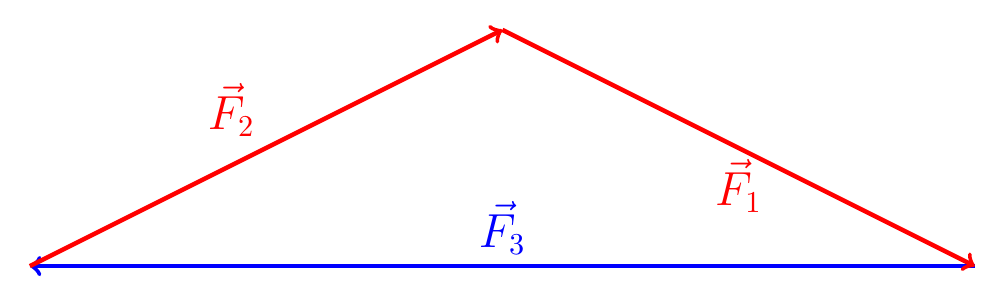
\begin{tikzpicture}[line width=0.7mm]
  \coordinate (v1) at (12,0);
  \coordinate (v3) at (0,0);
  \coordinate (v4) at (6,3);
  \coordinate (v5) at (6,-3);
  % add coordinate at the extension of the line from v1 to v2
 
  %o primeiro termo entre colchetes acima, seleciona o tamanho da fonte
  %já o último termo posiciona a figura
  \draw[blue,ultra thick,->]  (v1) -- node[font=\fontsize{16pt}{16pt}\selectfont,above] {$\vec{F_{3}}$}(v3);
  %rótulo das alturas,lados...
  \draw[red,ultra thick,->] (v4) --node[font=\fontsize{16pt}{16pt}\selectfont,below] {$\vec{F}_{1}$} (v1);
  \draw[red,ultra thick,->] (v3) --node[font=\fontsize{16pt}{16pt}\selectfont,above left] {$\vec{F}_{2}$} (v4);
\end{tikzpicture}


